\nocite{*}
\documentclass[a4paper, twoside]{report}

\usepackage[outdir=./]{epstopdf}

% Ancore
\usepackage{float}

% Dimensione dei margini
\usepackage[a4paper,top=3cm,bottom=3cm,left=3cm,right=3cm]{geometry} 
% Dimensione del font
\usepackage[fontsize=13pt]{scrextend}
% Lingua del testo
\usepackage[english]{babel}
% Lingua per la bibliografia
\usepackage[fixlanguage]{babelbib}
% Codifica del testo
\usepackage[utf8]{inputenc} 
% Encoding del testo
\usepackage[T1]{fontenc}
% Permette di generare testo fittizio. Mi è stato utile 
% per capire quale sarebbe stata l'impostazione del 
% testo nella pagina prima che scrivessi un determinato paragrafo
\usepackage{lipsum}
% Per ruotare le immagini
\usepackage{rotating}
% Per modificare l'header delle pagine 
\usepackage{fancyhdr}               

% Librerie matematiche
\usepackage{amssymb}
\usepackage{amsmath}
\usepackage{amsthm}         

% Uso delle immagini
\usepackage{graphicx}
% Uso dei colori
\usepackage[dvipsnames]{xcolor}         
% Uso dei listing per il codice
\usepackage{listings}          
% Per inserire gli hyperlinks tra i vari elementi del testo 
\usepackage{hyperref}     
% Diversi tipi di sottolineature
\usepackage[normalem]{ulem}

% -----------------------------------------------------------------

% Modifica lo stile dell'header
\pagestyle{fancy}
\fancyhf{}
\lhead{\rightmark}
\rhead{\textbf{\thepage}}
\fancyfoot{}
\setlength{\headheight}{12.5pt}

% Rimuove il numero di pagina all'inizio dei capitoli
\fancypagestyle{plain}{
  \fancyfoot{}
  \fancyhead{}
  \renewcommand{\headrulewidth}{0pt}
}

% Cambio carattere per monospaziato
\renewcommand{\ttdefault}{pcr}

% Stile del codice
\lstdefinestyle{codeStyle}{
    % Colore dei commenti
    commentstyle=\color{teal},
    % Colore delle keyword
    keywordstyle=\color{Magenta},
    % Stile dei numeri di riga
    numberstyle=\tiny\color{gray},
    % Colore delle stringhe
    stringstyle=\color{violet},
    % Dimensione e stile del testo
    basicstyle=\ttfamily\scriptsize,
    % newline solo ai whitespaces
    breakatwhitespace=false,     
    % newline si/no
    breaklines=true,                 
    % Posizione della caption, top/bottom 
    captionpos=b,                    
    % Mantiene gli spazi nel codice, utile per l'indentazione
    keepspaces=true,                 
    % Dove visualizzare i numeri di linea
    numbers=left,                    
    % Distanza tra i numeri di linea
    numbersep=5pt,                  
    % Mostra gli spazi bianchi o meno
    showspaces=false,                
    % Mostra gli spazi bianchi nelle stringhe
    showstringspaces=false,
    % Mostra i tab
    showtabs=false,
    % Dimensione dei tab
    tabsize=2,
    % accenti
    literate={á}{{\'a}}1 {à}{{\`a}}1 {é}{{\'e}}1 {è}{{\`e}}1,
    % wrap long lines on new line
    postbreak=\mbox{\textcolor{red}{$\hookrightarrow$}\space},
} \lstset{style=codeStyle}

% Stile di codice per dimensioni maggiori, in cui ho avuto bisogno di un testo più picolo (ad esempio se si vuole inserire del codice che ha linee molto lunghe). Per usare questo stile piuttosto che il precedente, usare 

% \lstset{style=longBlock}
%  % inserire il codice...
% \lstset{style=codeStyle}

% Il secondo comando consente di tornare allo stile precedente 
\lstdefinestyle{longBlock}{
    commentstyle=\color{teal},
    keywordstyle=\color{Magenta},
    numberstyle=\tiny\color{gray},
    stringstyle=\color{violet},
    basicstyle=\ttfamily\scriptsize,
    breakatwhitespace=false,         
    breaklines=true,                 
    captionpos=b,                    
    keepspaces=true,                 
    numbers=left,                    
    numbersep=5pt,                  
    showspaces=false,                
    showstringspaces=false,
    showtabs=false,                  
    tabsize=2
} \lstset{style=codeStyle}

% Togliendo il commento al comando che segue, si inseriscono nella bibliografia anche le fonti presenti in Bibliography.bib ma non citati direttamente con il comando \cite
% \nocite{*}

% Margini prima e dopo blocchi di codice, per avere più distanza
\lstset{aboveskip=20pt,belowskip=20pt}

% Modifica dello stile dei riferimenti, con il testo in cyano
\hypersetup{
    colorlinks,
    linkcolor=CornflowerBlue,
    citecolor=CornflowerBlue
}

% Aggiunti definizioni, teoremi, linea e listing
\newtheorem{definition}{Definizione}[section]
\newtheorem{theorem}{Teorema}[section]
\providecommand*\definitionautorefname{Definizione}
\providecommand*\theoremautorefname{Teorema}
\providecommand*{\listingautorefname}{Listing}
\providecommand*\lstnumberautorefname{Linea}

\raggedbottom


% -----------------------------------------------------------------
\begin{document}

\begin{titlepage}
    \begin{figure}[!htb]
        \centering
        
\includegraphics[keepaspectratio=true,scale=0.5]{images/Frontpage/cherubinFrontespizio.eps}
    \end{figure}
    
    \begin{center}
        \LARGE{UNIVERSITÀ DI PISA}
        \vspace{5mm}
        \\ \Large{SHREK GROUP}
        \vspace{5mm}
        \\ \LARGE{Cloud Computing Project}
    \end{center}
    
    \vspace{15mm}
    \begin{center}
        {\LARGE{\bf K-Means on MapReduce }}
        
        % Se il titolo è abbastanza corto da stare su una riga, si può usare
        
        % {\LARGE{\bf Un fantastico titolo per la mia tesi!}}
    \end{center}
    \vspace{30mm}
    
    \begin{minipage}[t]{0.47\textwidth}
        {\large{Members:}{
            \normalsize\vspace{3mm}\bf\\ \large{Matteo Pasqualetti} 
            \normalsize\vspace{3mm}\bf\\ \large{Daniele Giaquinta}
            \normalsize\vspace{3mm}\bf\\ \large{Francesco Londretti}}}
    \end{minipage}
    \hfill
    
    \vspace{30mm}
    \hrulefill
    
    \end{titlepage}

\tableofcontents

% Rimuovere se non si vuole la tabella delle figure
% \listoffigures

\chapter{Introduction}

Within the world of academic evaluations and certification procedures, ensuring the fairness and honesty of assessments 
has forever been a top priority. The reputation of educational institutions and the significance of certifications 
rely on the guarantee that the work submitted is authentic and the result of an individual's own endeavor. 
However, the emergence of highly sophisticated AI-driven language models has muddled the distinction between content 
created by humans and that generated by machines.

Imagine a situation where someone is competing for a highly respected certification. They submit a detailed essay, 
claiming it to be their own creation. However, what the examiners don't know is that the essay might have actually 
been written by a computer program. This discovery would immediately threaten the fairness of the certification process. 
It's not just a problem for the certification organization; it also diminishes the hard work of honest candidates who 
genuinely put in the effort to create their own content.

Moreover, the increase in online education and remote testing, hastened by unexpected global circumstances, 
has made it even harder to verify that students' work is truly their own. With traditional in-person supervision no 
longer possible, and the growing reliance on digital platforms for learning and assessment, there are now opportunities 
for individuals to misuse technology by either cheating or using AI models to complete their assignments. This situation 
adds to the complexity of the issue.

In this report, we will delve into the details of our approach, methodology, and the underlying principles of 
building the \textit{GPT Detection System}. We will also explore the implications and potential benefits of implementing 
this technology in educational settings, emphasizing its role in maintaining the integrity of assessment processes. 

\subsubsection{Alternative Uses}

While our main goal with the \textit{GPT Detection System} is to ensure the legitimacy of academic assessments, 
this technology has uses that reach far beyond the education sector. Its adaptability and precision unlock a wide array 
of potential applications in different fields. In the following sections, we'll delve into some exciting possibilities 
where the integration of this detection system could bring significant advantages:

\begin{itemize}
 \item \textbf{Content Moderation:} In the age of user-generated content, online platforms grapple with the challenge of 
    identifying and filtering out automated or malicious submissions. Our \textit{GPT Detection System} could assist 
    in automating the process of content moderation, ensuring that user-generated content aligns with community 
    guidelines and is free from automated spam or inappropriate material.
 \item \textbf{Fake News Detection:} Misinformation and fake news have become pervasive issues in the digital age. 
    Our technology can be employed to discern between legitimate news articles and those generated by automated systems, 
    contributing to the fight against the spread of false information.
 \item \textbf{Plagiarism Detection:} Beyond academia, our \textit{GPT Detection System} can be used by professional 
    writers, journalists, and content creators to ensure the originality of their work. 
    It can assist in identifying instances of content reuse and potential copyright violations.
 \item \textbf{Quality Control in Automated Content Generation:} Organizations that utilize AI models to generate content, 
    such as chatbots or automated customer service responses, can employ our detector to validate the authenticity 
    and quality of the generated responses, ensuring a seamless user experience.
 \item \textbf{Forensic Analysis:} Law enforcement agencies and forensic experts can utilize this technology to aid 
    in analyzing text-based evidence, verifying the authenticity of digital documents, and differentiating 
    between human and machine-generated text in criminal investigations.
 \item \textbf{Online Dating and Social Interaction:} In the realm of online dating and social networking, this detector 
    can help users verify the authenticity of profiles and messages, reducing the risk of encountering fraudulent 
    or automated interactions.
 \item \textbf{Content Creation Assistance:} Writers and content creators can use our tool to assess the authorship 
    of text, aiding in the identification of the original author or source of inspiration for research and creative writing.
 \item \textbf{Historical Text Analysis:} Historians and researchers can benefit from this detector when analyzing 
    historical texts and documents, helping to distinguish between text written by historical figures and potentially 
    forged or altered content.
\end{itemize}

The potential applications of our text classifier are expansive, transcending the boundaries of academia to address 
issues of authenticity, credibility, and trustworthiness in various sectors. As we delve into the methodology 
and implementation details, it becomes evident that this technology represents a powerful tool with far-reaching
implications for a wide range of fields and industries.
\chapter{Methodology}

\section{}

We used the \textit{zero-shot} method \cite{mitchell2023detectgpt}, that is  a way of detecting machine-generated text without using any labeled data or fine-tuning. It uses only the raw log probabilities computed by a generative model to determine if a candidate passage was sampled from it.

\begin{figure}[H]
	\centering
	\includegraphics[width=0.8\linewidth]{images/Methodology/plagiarized_paper_diagram}
	\caption{System's inner workings}
	\label{fig:plagiarizedpaperdiagram}
\end{figure}

The zero-shot method designed by Eric Mitchell et al. is called \textit{DetectGPT}. It's based on the hypothesis that samples from a source model typically lie in areas of negative curvature of the log probability function of the model, unlike human text. DetectGPT introduces random perturbations to the wording in a text sample and uses the changes in likelihood under an LLM as a discriminative signal.

\paragraph{How it works}
The system works as follows: it applies $N$ perturbations to the input text --- a perturbation is generated by making a encoder-decoder model, such as \textit{T5}, slightly rephrase the input text ---, it computes their log probability and computes a final metric, described by Formula \ref{formula:logprobmetric} that is compared to a certain $\varepsilon$ to determine if the input is from a GPT model.

\begin{figure}[H]
	\centering
	\label{formula:logprobmetric}
	\begin{equation}
		\dfrac{1}{N} \sum_{i = 0}^{N}
		\log\left(
		\dfrac{p(x)}{p(\tilde{x_i})}
		\right)
		\stackrel{?}{>}
		\varepsilon
	\end{equation}
\end{figure}

\paragraph{News article}
Currently, it seems this system might be the state-of-the-art for detecting GPT-generated texts \cite{state-of-the-art-article}.

\section{Drawbacks}

An assumption made is that we have a reasonable way to perturb the text and see how the probabilities change, we used \textit{T5} but some domains may have lower performance if this model doesn't capture the space of meaningful rephrases well, affecting the quality of the curvature estimate. Another problem is that the system is more computationally expensive than other detection methods, as it needs to sample and score the set of perturbations for each candidate passage, instead of just the candidate passage; a better way to perturb the text or estimate the curvature more efficiently may help reduce these costs.

It's also to be noted that the system may not be able to properly detect texts generated by \textit{large language models} other than the one used to compute the log probabilities.
\chapter{Application}

As we can see, the layout of the application is divided in two sections: the choice of the folder and the selected document.

In the first one we can choose the folder to scan and analyze, while in the second secion we can see the text and the
result of the detection.

%%%

We've recently developed a robust graphical application aimed at simplifying the document scanning process for 
organizations dealing with gpt-generated texts. This innovative tool streamlines batch processing tasks with just 
a few clicks, making it a valuable asset for any workflow.

\paragraph{Technology Stack} Our application is built using Python and relies on the Qt5 framework, which is known 
for its cross-platform compatibility, to create an intuitive and user-friendly graphical interface.

\section{Layout and Features}

\paragraph{Folder Selection} One of the key features of our application is the ability to effortlessly select the 
target folder for document scanning and analysis. This ensures that users can easily pinpoint the location of the 
documents they want to process.

\paragraph{Document Preview} In the second section of the application, users are presented with a comprehensive 
view of the selected document. Here, they can examine the extracted text and view the results of the detection process.

\paragraph{Efficiency and Accuracy} Our application employs state-of-the-art algorithms to detect gpt-written 
text within documents. This ensures both efficiency and accuracy in identifying and processing relevant content.

\paragraph{Batch Processing} The real strength of our application lies in its batch processing capabilities. 
Users can queue up multiple documents within a selected folder, allowing for simultaneous scanning and analysis. 
This significantly reduces the time and effort required for handling a large number of documents.

\paragraph{User-Friendly Interface} With a focus on usability, our application boasts an intuitive interface. 
Even those with limited technical expertise can navigate through the process with ease, thanks to its simple and 
straightforward design.

\paragraph{Visual Aid} To provide a clearer picture of the application, we've included an image below that showcases 
its layout and features.

\begin{figure}
	\centering
	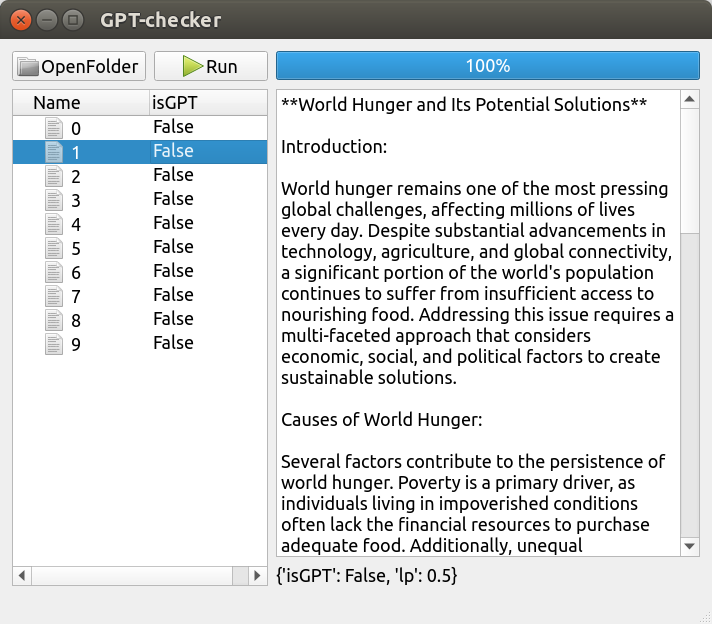
\includegraphics[width=0.8\linewidth]{images/Application/screen}
	\caption{Application's main window}
	\label{fig:screen}
\end{figure}


In conclusion, our innovative document scanning application powered by Python and Qt5 offers organizations a 
convenient and efficient solution for identifying and processing gpt-generated texts. Its user-friendly 
interface and batch processing capabilities make it an indispensable tool for enhancing productivity and accuracy 
in document management tasks.

%%%
\chapter{Conclusion}

\appendix

\include{chapters/AppendixA}

\bibliographystyle{plain}
\bibliography{chapters/Bibliografy.bib}

\end{document}
% -----------------------------------------------------------------
